\documentclass[1p]{elsarticle_modified}
%\bibliographystyle{elsarticle-num}

%\usepackage[colorlinks]{hyperref}
%\usepackage{abbrmath_seonhwa} %\Abb, \Ascr, \Acal ,\Abf, \Afrak
\usepackage{amsfonts}
\usepackage{amssymb}
\usepackage{amsmath}
\usepackage{amsthm}
\usepackage{scalefnt}
\usepackage{amsbsy}
\usepackage{kotex}
\usepackage{caption}
\usepackage{subfig}
\usepackage{color}
\usepackage{graphicx}
\usepackage{xcolor} %% white, black, red, green, blue, cyan, magenta, yellow
\usepackage{float}
\usepackage{setspace}
\usepackage{hyperref}

\usepackage{tikz}
\usetikzlibrary{arrows}

\usepackage{multirow}
\usepackage{array} % fixed length table
\usepackage{hhline}

%%%%%%%%%%%%%%%%%%%%%
\makeatletter
\renewcommand*\env@matrix[1][\arraystretch]{%
	\edef\arraystretch{#1}%
	\hskip -\arraycolsep
	\let\@ifnextchar\new@ifnextchar
	\array{*\c@MaxMatrixCols c}}
\makeatother %https://tex.stackexchange.com/questions/14071/how-can-i-increase-the-line-spacing-in-a-matrix
%%%%%%%%%%%%%%%

\usepackage[normalem]{ulem}

\newcommand{\msout}[1]{\ifmmode\text{\sout{\ensuremath{#1}}}\else\sout{#1}\fi}
%SOURCE: \msout is \stkout macro in https://tex.stackexchange.com/questions/20609/strikeout-in-math-mode

\newcommand{\cancel}[1]{
	\ifmmode
	{\color{red}\msout{#1}}
	\else
	{\color{red}\sout{#1}}
	\fi
}

\newcommand{\add}[1]{
	{\color{blue}\uwave{#1}}
}

\newcommand{\replace}[2]{
	\ifmmode
	{\color{red}\msout{#1}}{\color{blue}\uwave{#2}}
	\else
	{\color{red}\sout{#1}}{\color{blue}\uwave{#2}}
	\fi
}

\newcommand{\Sol}{\mathcal{S}} %segment
\newcommand{\D}{D} %diagram
\newcommand{\A}{\mathcal{A}} %arc


%%%%%%%%%%%%%%%%%%%%%%%%%%%%%5 test

\def\sl{\operatorname{\textup{SL}}(2,\Cbb)}
\def\psl{\operatorname{\textup{PSL}}(2,\Cbb)}
\def\quan{\mkern 1mu \triangleright \mkern 1mu}

\theoremstyle{definition}
\newtheorem{thm}{Theorem}[section]
\newtheorem{prop}[thm]{Proposition}
\newtheorem{lem}[thm]{Lemma}
\newtheorem{ques}[thm]{Question}
\newtheorem{cor}[thm]{Corollary}
\newtheorem{defn}[thm]{Definition}
\newtheorem{exam}[thm]{Example}
\newtheorem{rmk}[thm]{Remark}
\newtheorem{alg}[thm]{Algorithm}

\newcommand{\I}{\sqrt{-1}}
\begin{document}

%\begin{frontmatter}
%
%\title{Boundary parabolic representations of knots up to 8 crossings}
%
%%% Group authors per affiliation:
%\author{Yunhi Cho} 
%\address{Department of Mathematics, University of Seoul, Seoul, Korea}
%\ead{yhcho@uos.ac.kr}
%
%
%\author{Seonhwa Kim} %\fnref{s_kim}}
%\address{Center for Geometry and Physics, Institute for Basic Science, Pohang, 37673, Korea}
%\ead{ryeona17@ibs.re.kr}
%
%\author{Hyuk Kim}
%\address{Department of Mathematical Sciences, Seoul National University, Seoul 08826, Korea}
%\ead{hyukkim@snu.ac.kr}
%
%\author{Seokbeom Yoon}
%\address{Department of Mathematical Sciences, Seoul National University, Seoul, 08826,  Korea}
%\ead{sbyoon15@snu.ac.kr}
%
%\begin{abstract}
%We find all boundary parabolic representation of knots up to 8 crossings.
%
%\end{abstract}
%\begin{keyword}
%    \MSC[2010] 57M25 
%\end{keyword}
%
%\end{frontmatter}

%\linenumbers
%\tableofcontents
%
\newcommand\colored[1]{\textcolor{white}{\rule[-0.35ex]{0.8em}{1.4ex}}\kern-0.8em\color{red} #1}%
%\newcommand\colored[1]{\textcolor{white}{ #1}\kern-2.17ex	\textcolor{white}{ #1}\kern-1.81ex	\textcolor{white}{ #1}\kern-2.15ex\color{red}#1	}

{\Large $\underline{12n_{0847}~(K12n_{0847})}$}

\setlength{\tabcolsep}{10pt}
\renewcommand{\arraystretch}{1.6}
\vspace{1cm}\begin{tabular}{m{100pt}>{\centering\arraybackslash}m{274pt}}
\multirow{5}{120pt}{
	\centering
	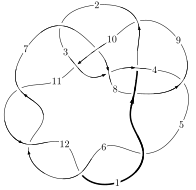
\includegraphics[width=112pt]{../../../GIT/diagram.site/Diagrams/png/2936_12n_0847.png}\\
\ \ \ A knot diagram\footnotemark}&
\allowdisplaybreaks
\textbf{Linearized knot diagam} \\
\cline{2-2}
 &
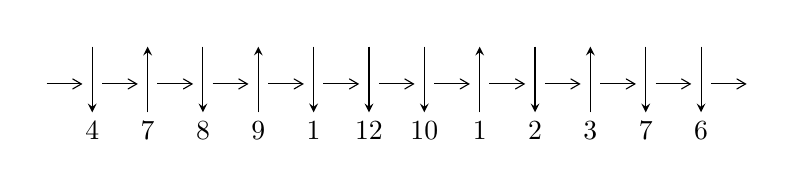
\begin{tikzpicture}[x=20pt, y=17pt]
	% nodes
	\node (C0) at (0, 0) {};
	\node (C1) at (1, 0) {};
	\node (C1U) at (1, +1) {};
	\node (C1D) at (1, -1) {4};

	\node (C2) at (2, 0) {};
	\node (C2U) at (2, +1) {};
	\node (C2D) at (2, -1) {7};

	\node (C3) at (3, 0) {};
	\node (C3U) at (3, +1) {};
	\node (C3D) at (3, -1) {8};

	\node (C4) at (4, 0) {};
	\node (C4U) at (4, +1) {};
	\node (C4D) at (4, -1) {9};

	\node (C5) at (5, 0) {};
	\node (C5U) at (5, +1) {};
	\node (C5D) at (5, -1) {1};

	\node (C6) at (6, 0) {};
	\node (C6U) at (6, +1) {};
	\node (C6D) at (6, -1) {12};

	\node (C7) at (7, 0) {};
	\node (C7U) at (7, +1) {};
	\node (C7D) at (7, -1) {10};

	\node (C8) at (8, 0) {};
	\node (C8U) at (8, +1) {};
	\node (C8D) at (8, -1) {1};

	\node (C9) at (9, 0) {};
	\node (C9U) at (9, +1) {};
	\node (C9D) at (9, -1) {2};

	\node (C10) at (10, 0) {};
	\node (C10U) at (10, +1) {};
	\node (C10D) at (10, -1) {3};

	\node (C11) at (11, 0) {};
	\node (C11U) at (11, +1) {};
	\node (C11D) at (11, -1) {7};

	\node (C12) at (12, 0) {};
	\node (C12U) at (12, +1) {};
	\node (C12D) at (12, -1) {6};
	\node (C13) at (13, 0) {};

	% arrows
	\draw[->,>={angle 60}]
	(C0) edge (C1) (C1) edge (C2) (C2) edge (C3) (C3) edge (C4) (C4) edge (C5) (C5) edge (C6) (C6) edge (C7) (C7) edge (C8) (C8) edge (C9) (C9) edge (C10) (C10) edge (C11) (C11) edge (C12) (C12) edge (C13) ;	\draw[->,>=stealth]
	(C1U) edge (C1D) (C2D) edge (C2U) (C3U) edge (C3D) (C4D) edge (C4U) (C5U) edge (C5D) (C6U) edge (C6D) (C7U) edge (C7D) (C8D) edge (C8U) (C9U) edge (C9D) (C10D) edge (C10U) (C11U) edge (C11D) (C12U) edge (C12D) ;
	\end{tikzpicture} \\
\hhline{~~} \\& 
\textbf{Solving Sequence} \\ \cline{2-2} 
 &
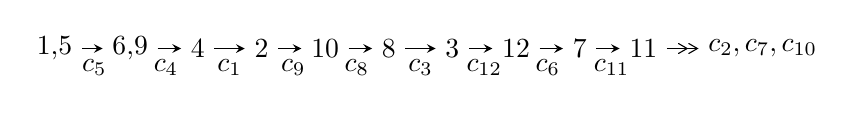
\begin{tikzpicture}[x=23pt, y=7pt]
	% node
	\node (A0) at (-1/8, 0) {1,5};
	\node (A1) at (17/16, 0) {6,9};
	\node (A2) at (17/8, 0) {4};
	\node (A3) at (25/8, 0) {2};
	\node (A4) at (33/8, 0) {10};
	\node (A5) at (41/8, 0) {8};
	\node (A6) at (49/8, 0) {3};
	\node (A7) at (57/8, 0) {12};
	\node (A8) at (65/8, 0) {7};
	\node (A9) at (73/8, 0) {11};
	\node (C1) at (1/2, -1) {$c_{5}$};
	\node (C2) at (13/8, -1) {$c_{4}$};
	\node (C3) at (21/8, -1) {$c_{1}$};
	\node (C4) at (29/8, -1) {$c_{9}$};
	\node (C5) at (37/8, -1) {$c_{8}$};
	\node (C6) at (45/8, -1) {$c_{3}$};
	\node (C7) at (53/8, -1) {$c_{12}$};
	\node (C8) at (61/8, -1) {$c_{6}$};
	\node (C9) at (69/8, -1) {$c_{11}$};
	\node (A10) at (11, 0) {$c_{2},c_{7},c_{10}$};

	% edge
	\draw[->,>=stealth]	
	(A0) edge (A1) (A1) edge (A2) (A2) edge (A3) (A3) edge (A4) (A4) edge (A5) (A5) edge (A6) (A6) edge (A7) (A7) edge (A8) (A8) edge (A9) ;
	\draw[->>,>={angle 60}]	
	(A9) edge (A10);
\end{tikzpicture} \\ 

\end{tabular} \\

\footnotetext{
The image of knot diagram is generated by the software ``\textbf{Draw programme}" developed by Andrew Bartholomew(\url{http://www.layer8.co.uk/maths/draw/index.htm\#Running-draw}), where we modified some parts for our purpose(\url{https://github.com/CATsTAILs/LinksPainter}).
}\phantom \\ \newline 
\centering \textbf{Ideals for irreducible components\footnotemark of $X_{\text{par}}$} 
 
\begin{align*}
I^u_{1}&=\langle 
3 u^{10}-5 u^9-28 u^8-131 u^7-313 u^6-576 u^5-809 u^4-779 u^3-575 u^2+58 b-246 u-70,\\
\phantom{I^u_{1}}&\phantom{= \langle  }-35 u^{10}-222 u^9+\cdots+232 a-556,\\
\phantom{I^u_{1}}&\phantom{= \langle  }u^{11}+6 u^{10}+23 u^9+62 u^8+128 u^7+210 u^6+269 u^5+270 u^4+202 u^3+108 u^2+44 u+8\rangle \\
I^u_{2}&=\langle 
a u+b,\;8 u^6 a-3 u^6+\cdots+28 a-18,\;u^7+4 u^6+11 u^5+20 u^4+26 u^3+25 u^2+14 u+4\rangle \\
I^u_{3}&=\langle 
- a^3 u+2 a^3-7 a^2 u+5 a^2-12 a u+6 b-9 u-9,\;a^4-2 a^3 u+3 a^3-4 a^2 u+3 a^2-7 a u+2 a-2 u+1,\\
\phantom{I^u_{3}}&\phantom{= \langle  }u^2- u+1\rangle \\
I^u_{4}&=\langle 
- a u+b- u,\;a^2+a-2 u+2,\;u^2- u+1\rangle \\
I^u_{5}&=\langle 
u^{12}- u^{11}+8 u^{10}-8 u^9+25 u^8-24 u^7+42 u^6-36 u^5+42 u^4-31 u^3+22 u^2+2 b-13 u+5,\\
\phantom{I^u_{5}}&\phantom{= \langle  }-5 u^{15}-55 u^{13}+\cdots+38 a-247,\;u^{16}+11 u^{14}+51 u^{12}+134 u^{10}+226 u^8+256 u^6+191 u^4+88 u^2+19\rangle \\
I^u_{6}&=\langle 
a^3 u+a^3+a^2 u-5 a^2-6 a u+3 b+3 a+6 u+3,\;a^4+a^3 u-3 a^3-2 a^2 u+2 a^2+2 a u+2 a- u-1,\\
\phantom{I^u_{6}}&\phantom{= \langle  }u^2- u+1\rangle \\
I^u_{7}&=\langle 
- a u+b+u-1,\;a^2- a u-2 u+1,\;u^2- u+1\rangle \\
I^u_{8}&=\langle 
b- u+1,\;a-1,\;u^2- u+1\rangle \\
I^u_{9}&=\langle 
b+u,\;a+u,\;u^2- u+1\rangle \\
I^u_{10}&=\langle 
b+u+1,\;a+u,\;u^2+u+1\rangle \\
\\
I^v_{1}&=\langle 
a,\;b^2+b+1,\;v+1\rangle \\
\end{align*}
\raggedright * 11 irreducible components of $\dim_{\mathbb{C}}=0$, with total 73 representations.\\
\footnotetext{All coefficients of polynomials are rational numbers. But the coefficients are sometimes approximated in decimal forms when there is not enough margin.}
\newpage
\renewcommand{\arraystretch}{1}
\centering \section*{I. $I^u_{1}= \langle 3 u^{10}-5 u^9+\cdots+58 b-70,\;-35 u^{10}-222 u^9+\cdots+232 a-556,\;u^{11}+6 u^{10}+\cdots+44 u+8 \rangle$}
\flushleft \textbf{(i) Arc colorings}\\
\begin{tabular}{m{7pt} m{180pt} m{7pt} m{180pt} }
\flushright $a_{1}=$&$\begin{pmatrix}0\\u\end{pmatrix}$ \\
\flushright $a_{5}=$&$\begin{pmatrix}1\\0\end{pmatrix}$ \\
\flushright $a_{6}=$&$\begin{pmatrix}1\\u^2\end{pmatrix}$ \\
\flushright $a_{9}=$&$\begin{pmatrix}0.150862 u^{10}+0.956897 u^{9}+\cdots+6.37931 u+2.39655\\-0.0517241 u^{10}+0.0862069 u^{9}+\cdots+4.24138 u+1.20690\end{pmatrix}$ \\
\flushright $a_{4}=$&$\begin{pmatrix}0.314655 u^{10}+1.51724 u^{9}+\cdots+9.94828 u+3.74138\\0.370690 u^{10}+1.96552 u^{9}+\cdots+11.1034 u+2.51724\end{pmatrix}$ \\
\flushright $a_{2}=$&$\begin{pmatrix}-0.193966 u^{10}-0.801724 u^{9}+\cdots-1.34483 u+0.775862\\-0.620690 u^{10}-3.46552 u^{9}+\cdots-22.1034 u-4.51724\end{pmatrix}$ \\
\flushright $a_{10}=$&$\begin{pmatrix}0.150862 u^{10}+0.706897 u^{9}+\cdots+4.87931 u+1.39655\\0.698276 u^{10}+2.58621 u^{9}+\cdots+12.2414 u+3.20690\end{pmatrix}$ \\
\flushright $a_{8}=$&$\begin{pmatrix}0.150862 u^{10}+0.956897 u^{9}+\cdots+6.37931 u+2.39655\\-0.448276 u^{10}-1.58621 u^{9}+\cdots+0.758621 u+0.793103\end{pmatrix}$ \\
\flushright $a_{3}=$&$\begin{pmatrix}0.564655 u^{10}+2.76724 u^{9}+\cdots+11.4483 u+2.74138\\0.620690 u^{10}+3.46552 u^{9}+\cdots+32.1034 u+6.51724\end{pmatrix}$ \\
\flushright $a_{12}=$&$\begin{pmatrix}u\\u^3+u\end{pmatrix}$ \\
\flushright $a_{7}=$&$\begin{pmatrix}u^2+1\\u^4+2 u^2\end{pmatrix}$ \\
\flushright $a_{11}=$&$\begin{pmatrix}u^3+2 u\\u^5+3 u^3+u\end{pmatrix}$\\&\end{tabular}
\flushleft \textbf{(ii) Obstruction class $= -1$}\\~\\
\flushleft \textbf{(iii) Cusp Shapes $= -\frac{55}{58} u^{10}-\frac{162}{29} u^9-\frac{1217}{58} u^8-\frac{1588}{29} u^7-\frac{3216}{29} u^6-\frac{5073}{29} u^5-\frac{12583}{58} u^4-\frac{5972}{29} u^3-\frac{4159}{29} u^2-\frac{2124}{29} u-\frac{702}{29}$}\\~\\
\newpage\renewcommand{\arraystretch}{1}
\flushleft \textbf{(iv) u-Polynomials at the component}\newline \\
\begin{tabular}{m{50pt}|m{274pt}}
Crossings & \hspace{64pt}u-Polynomials at each crossing \\
\hline $$\begin{aligned}c_{1},c_{7}\end{aligned}$$&$\begin{aligned}
&u^{11}-5 u^{10}+\cdots+5 u+7
\end{aligned}$\\
\hline $$\begin{aligned}c_{2},c_{4},c_{8}\\c_{10}\end{aligned}$$&$\begin{aligned}
&u^{11}+u^{10}+6 u^9+4 u^8+14 u^7+4 u^6+8 u^5-5 u^3-3 u^2+u+1
\end{aligned}$\\
\hline $$\begin{aligned}c_{3},c_{9}\end{aligned}$$&$\begin{aligned}
&u^{11}-2 u^{10}+\cdots-9 u+24
\end{aligned}$\\
\hline $$\begin{aligned}c_{5},c_{6},c_{11}\\c_{12}\end{aligned}$$&$\begin{aligned}
&u^{11}+6 u^{10}+\cdots+44 u+8
\end{aligned}$\\
\hline
\end{tabular}\\~\\
\newpage\renewcommand{\arraystretch}{1}
\flushleft \textbf{(v) Riley Polynomials at the component}\newline \\
\begin{tabular}{m{50pt}|m{274pt}}
Crossings & \hspace{64pt}Riley Polynomials at each crossing \\
\hline $$\begin{aligned}c_{1},c_{7}\end{aligned}$$&$\begin{aligned}
&y^{11}+5 y^{10}+\cdots-31 y-49
\end{aligned}$\\
\hline $$\begin{aligned}c_{2},c_{4},c_{8}\\c_{10}\end{aligned}$$&$\begin{aligned}
&y^{11}+11 y^{10}+\cdots+7 y-1
\end{aligned}$\\
\hline $$\begin{aligned}c_{3},c_{9}\end{aligned}$$&$\begin{aligned}
&y^{11}-22 y^{10}+\cdots+4305 y-576
\end{aligned}$\\
\hline $$\begin{aligned}c_{5},c_{6},c_{11}\\c_{12}\end{aligned}$$&$\begin{aligned}
&y^{11}+10 y^{10}+\cdots+208 y-64
\end{aligned}$\\
\hline
\end{tabular}\\~\\
\newpage\flushleft \textbf{(vi) Complex Volumes and Cusp Shapes}
$$\begin{array}{c|c|c}  
\text{Solutions to }I^u_{1}& \I (\text{vol} + \sqrt{-1}CS) & \text{Cusp shape}\\
 \hline 
\begin{aligned}
u &= -0.077559 + 0.704837 I \\
a &= \phantom{-}0.121802 - 0.808314 I \\
b &= -0.560282 - 0.148542 I\end{aligned}
 & \phantom{-}0.79523 + 1.67374 I & \phantom{-}1.92464 - 5.47847 I \\ \hline\begin{aligned}
u &= -0.077559 - 0.704837 I \\
a &= \phantom{-}0.121802 + 0.808314 I \\
b &= -0.560282 + 0.148542 I\end{aligned}
 & \phantom{-}0.79523 - 1.67374 I & \phantom{-}1.92464 + 5.47847 I \\ \hline\begin{aligned}
u &= -1.377920 + 0.101637 I \\
a &= -0.324451 + 1.135490 I \\
b &= -0.33166 + 1.59759 I\end{aligned}
 & -11.42710 - 8.15511 I & -7.08884 + 4.54839 I \\ \hline\begin{aligned}
u &= -1.377920 - 0.101637 I \\
a &= -0.324451 - 1.135490 I \\
b &= -0.33166 - 1.59759 I\end{aligned}
 & -11.42710 + 8.15511 I & -7.08884 - 4.54839 I \\ \hline\begin{aligned}
u &= -0.72850 + 1.42389 I \\
a &= -0.649822 + 0.893927 I \\
b &= \phantom{-}0.79946 + 1.57650 I\end{aligned}
 & -7.3754 + 15.4551 I & -4.41387 - 7.80880 I \\ \hline\begin{aligned}
u &= -0.72850 - 1.42389 I \\
a &= -0.649822 - 0.893927 I \\
b &= \phantom{-}0.79946 - 1.57650 I\end{aligned}
 & -7.3754 - 15.4551 I & -4.41387 + 7.80880 I \\ \hline\begin{aligned}
u &= -0.361176\phantom{ +0.000000I} \\
a &= \phantom{-}1.44545\phantom{ +0.000000I} \\
b &= \phantom{-}0.522063\phantom{ +0.000000I}\end{aligned}
 & -1.26726\phantom{ +0.000000I} & -9.58390\phantom{ +0.000000I} \\ \hline\begin{aligned}
u &= \phantom{-}0.08198 + 1.70897 I \\
a &= -0.264638 + 0.259315 I \\
b &= \phantom{-}0.464855 + 0.430999 I\end{aligned}
 & \phantom{-}9.26814 + 1.07224 I & \phantom{-}1.58191 - 6.79260 I \\ \hline\begin{aligned}
u &= \phantom{-}0.08198 - 1.70897 I \\
a &= -0.264638 - 0.259315 I \\
b &= \phantom{-}0.464855 - 0.430999 I\end{aligned}
 & \phantom{-}9.26814 - 1.07224 I & \phantom{-}1.58191 + 6.79260 I \\ \hline\begin{aligned}
u &= -0.71742 + 1.60214 I \\
a &= \phantom{-}0.644383 - 0.371812 I \\
b &= -0.133405 - 1.299140 I\end{aligned}
 & -6.25408 - 0.69480 I & -6.21186 + 0.79724 I\\
 \hline 
 \end{array}$$\newpage$$\begin{array}{c|c|c}  
\text{Solutions to }I^u_{1}& \I (\text{vol} + \sqrt{-1}CS) & \text{Cusp shape}\\
 \hline 
\begin{aligned}
u &= -0.71742 - 1.60214 I \\
a &= \phantom{-}0.644383 + 0.371812 I \\
b &= -0.133405 + 1.299140 I\end{aligned}
 & -6.25408 + 0.69480 I & -6.21186 - 0.79724 I\\
 \hline 
 \end{array}$$\newpage\newpage\renewcommand{\arraystretch}{1}
\centering \section*{II. $I^u_{2}= \langle a u+b,\;8 u^6 a-3 u^6+\cdots+28 a-18,\;u^7+4 u^6+\cdots+14 u+4 \rangle$}
\flushleft \textbf{(i) Arc colorings}\\
\begin{tabular}{m{7pt} m{180pt} m{7pt} m{180pt} }
\flushright $a_{1}=$&$\begin{pmatrix}0\\u\end{pmatrix}$ \\
\flushright $a_{5}=$&$\begin{pmatrix}1\\0\end{pmatrix}$ \\
\flushright $a_{6}=$&$\begin{pmatrix}1\\u^2\end{pmatrix}$ \\
\flushright $a_{9}=$&$\begin{pmatrix}a\\- a u\end{pmatrix}$ \\
\flushright $a_{4}=$&$\begin{pmatrix}-\frac{1}{2} u^6 a-2 u^5 a+\cdots-4 a+\frac{5}{2}\\-\frac{1}{2} u^6- u^5+\cdots-2 a-\frac{3}{2} u\end{pmatrix}$ \\
\flushright $a_{2}=$&$\begin{pmatrix}-\frac{1}{2} u^6-\frac{3}{2} u^5+\cdots- a-\frac{3}{2}\\\frac{1}{2} u^6+u^5+\cdots- a u+\frac{5}{2} u\end{pmatrix}$ \\
\flushright $a_{10}=$&$\begin{pmatrix}-\frac{1}{2} u^6 a+\frac{1}{4} u^6+\cdots+\frac{21}{4} u+\frac{5}{2}\\- u^6 a-3 u^5 a+\cdots-2 a-1\end{pmatrix}$ \\
\flushright $a_{8}=$&$\begin{pmatrix}a\\u^2 a- a u\end{pmatrix}$ \\
\flushright $a_{3}=$&$\begin{pmatrix}\frac{1}{2} u^5+u^4+\cdots- a+\frac{5}{2}\\- u^5 a-\frac{1}{2} u^6+\cdots- a u-\frac{3}{2} u\end{pmatrix}$ \\
\flushright $a_{12}=$&$\begin{pmatrix}u\\u^3+u\end{pmatrix}$ \\
\flushright $a_{7}=$&$\begin{pmatrix}u^2+1\\u^4+2 u^2\end{pmatrix}$ \\
\flushright $a_{11}=$&$\begin{pmatrix}u^3+2 u\\u^5+3 u^3+u\end{pmatrix}$\\&\end{tabular}
\flushleft \textbf{(ii) Obstruction class $= -1$}\\~\\
\flushleft \textbf{(iii) Cusp Shapes $= - u^6-3 u^5-11 u^4-21 u^3-30 u^2-28 u-14$}\\~\\
\newpage\renewcommand{\arraystretch}{1}
\flushleft \textbf{(iv) u-Polynomials at the component}\newline \\
\begin{tabular}{m{50pt}|m{274pt}}
Crossings & \hspace{64pt}u-Polynomials at each crossing \\
\hline $$\begin{aligned}c_{1},c_{7}\end{aligned}$$&$\begin{aligned}
&u^{14}-8 u^{13}+\cdots-21 u+3
\end{aligned}$\\
\hline $$\begin{aligned}c_{2},c_{4},c_{8}\\c_{10}\end{aligned}$$&$\begin{aligned}
&u^{14}+8 u^{12}+\cdots-3 u+1
\end{aligned}$\\
\hline $$\begin{aligned}c_{3},c_{9}\end{aligned}$$&$\begin{aligned}
&(u^7+u^6-2 u^5-2 u^4- u^3-3 u^2-1)^2
\end{aligned}$\\
\hline $$\begin{aligned}c_{5},c_{6},c_{11}\\c_{12}\end{aligned}$$&$\begin{aligned}
&(u^7+4 u^6+11 u^5+20 u^4+26 u^3+25 u^2+14 u+4)^2
\end{aligned}$\\
\hline
\end{tabular}\\~\\
\newpage\renewcommand{\arraystretch}{1}
\flushleft \textbf{(v) Riley Polynomials at the component}\newline \\
\begin{tabular}{m{50pt}|m{274pt}}
Crossings & \hspace{64pt}Riley Polynomials at each crossing \\
\hline $$\begin{aligned}c_{1},c_{7}\end{aligned}$$&$\begin{aligned}
&y^{14}+2 y^{13}+\cdots-33 y+9
\end{aligned}$\\
\hline $$\begin{aligned}c_{2},c_{4},c_{8}\\c_{10}\end{aligned}$$&$\begin{aligned}
&y^{14}+16 y^{13}+\cdots-3 y+1
\end{aligned}$\\
\hline $$\begin{aligned}c_{3},c_{9}\end{aligned}$$&$\begin{aligned}
&(y^7-5 y^6+6 y^5+6 y^4-9 y^3-13 y^2-6 y-1)^2
\end{aligned}$\\
\hline $$\begin{aligned}c_{5},c_{6},c_{11}\\c_{12}\end{aligned}$$&$\begin{aligned}
&(y^7+6 y^6+13 y^5-48 y^3-57 y^2-4 y-16)^2
\end{aligned}$\\
\hline
\end{tabular}\\~\\
\newpage\flushleft \textbf{(vi) Complex Volumes and Cusp Shapes}
$$\begin{array}{c|c|c}  
\text{Solutions to }I^u_{2}& \I (\text{vol} + \sqrt{-1}CS) & \text{Cusp shape}\\
 \hline 
\begin{aligned}
u &= -0.532984 + 0.464109 I \\
a &= \phantom{-}0.595528 - 0.213565 I \\
b &= \phantom{-}0.218289 - 0.390217 I\end{aligned}
 & -0.57333 + 1.84126 I & -2.97768 - 3.50098 I \\ \hline\begin{aligned}
u &= -0.532984 + 0.464109 I \\
a &= \phantom{-}0.58819 - 1.42915 I \\
b &= -0.349784 - 1.034700 I\end{aligned}
 & -0.57333 + 1.84126 I & -2.97768 - 3.50098 I \\ \hline\begin{aligned}
u &= -0.532984 - 0.464109 I \\
a &= \phantom{-}0.595528 + 0.213565 I \\
b &= \phantom{-}0.218289 + 0.390217 I\end{aligned}
 & -0.57333 - 1.84126 I & -2.97768 + 3.50098 I \\ \hline\begin{aligned}
u &= -0.532984 - 0.464109 I \\
a &= \phantom{-}0.58819 + 1.42915 I \\
b &= -0.349784 + 1.034700 I\end{aligned}
 & -0.57333 - 1.84126 I & -2.97768 + 3.50098 I \\ \hline\begin{aligned}
u &= -1.33180\phantom{ +0.000000I} \\
a &= \phantom{-}0.228400 + 1.212910 I \\
b &= \phantom{-}0.30418 + 1.61536 I\end{aligned}
 & -12.0300\phantom{ +0.000000I} & -7.93040\phantom{ +0.000000I} \\ \hline\begin{aligned}
u &= -1.33180\phantom{ +0.000000I} \\
a &= \phantom{-}0.228400 - 1.212910 I \\
b &= \phantom{-}0.30418 - 1.61536 I\end{aligned}
 & -12.0300\phantom{ +0.000000I} & -7.93040\phantom{ +0.000000I} \\ \hline\begin{aligned}
u &= -0.11506 + 1.49422 I \\
a &= -0.755700 + 0.587068 I \\
b &= \phantom{-}0.79026 + 1.19673 I\end{aligned}
 & \phantom{-}5.82905 + 4.07787 I & \phantom{-}5.41510 + 4.51647 I \\ \hline\begin{aligned}
u &= -0.11506 + 1.49422 I \\
a &= -0.095547 - 0.221715 I \\
b &= -0.342285 + 0.117257 I\end{aligned}
 & \phantom{-}5.82905 + 4.07787 I & \phantom{-}5.41510 + 4.51647 I \\ \hline\begin{aligned}
u &= -0.11506 - 1.49422 I \\
a &= -0.755700 - 0.587068 I \\
b &= \phantom{-}0.79026 - 1.19673 I\end{aligned}
 & \phantom{-}5.82905 - 4.07787 I & \phantom{-}5.41510 - 4.51647 I \\ \hline\begin{aligned}
u &= -0.11506 - 1.49422 I \\
a &= -0.095547 + 0.221715 I \\
b &= -0.342285 - 0.117257 I\end{aligned}
 & \phantom{-}5.82905 - 4.07787 I & \phantom{-}5.41510 - 4.51647 I\\
 \hline 
 \end{array}$$\newpage$$\begin{array}{c|c|c}  
\text{Solutions to }I^u_{2}& \I (\text{vol} + \sqrt{-1}CS) & \text{Cusp shape}\\
 \hline 
\begin{aligned}
u &= -0.68606 + 1.48551 I \\
a &= \phantom{-}0.668554 - 0.820572 I \\
b &= -0.76030 - 1.55610 I\end{aligned}
 & -7.46541 + 7.10242 I & -5.97220 - 3.89199 I \\ \hline\begin{aligned}
u &= -0.68606 + 1.48551 I \\
a &= -0.729428 + 0.430875 I \\
b &= \phantom{-}0.139642 + 1.379180 I\end{aligned}
 & -7.46541 + 7.10242 I & -5.97220 - 3.89199 I \\ \hline\begin{aligned}
u &= -0.68606 - 1.48551 I \\
a &= \phantom{-}0.668554 + 0.820572 I \\
b &= -0.76030 + 1.55610 I\end{aligned}
 & -7.46541 - 7.10242 I & -5.97220 + 3.89199 I \\ \hline\begin{aligned}
u &= -0.68606 - 1.48551 I \\
a &= -0.729428 - 0.430875 I \\
b &= \phantom{-}0.139642 - 1.379180 I\end{aligned}
 & -7.46541 - 7.10242 I & -5.97220 + 3.89199 I\\
 \hline 
 \end{array}$$\newpage\newpage\renewcommand{\arraystretch}{1}
\centering \section*{III. $I^u_{3}= \langle - a^3 u-7 a^2 u+\cdots+5 a^2-9,\;-2 a^3 u-4 a^2 u+\cdots+2 a+1,\;u^2- u+1 \rangle$}
\flushleft \textbf{(i) Arc colorings}\\
\begin{tabular}{m{7pt} m{180pt} m{7pt} m{180pt} }
\flushright $a_{1}=$&$\begin{pmatrix}0\\u\end{pmatrix}$ \\
\flushright $a_{5}=$&$\begin{pmatrix}1\\0\end{pmatrix}$ \\
\flushright $a_{6}=$&$\begin{pmatrix}1\\u-1\end{pmatrix}$ \\
\flushright $a_{9}=$&$\begin{pmatrix}a\\\frac{1}{6} a^3 u+\frac{7}{6} a^2 u+\cdots-\frac{5}{6} a^2+\frac{3}{2}\end{pmatrix}$ \\
\flushright $a_{4}=$&$\begin{pmatrix}\frac{1}{3} a^3 u+\frac{5}{6} a^2 u+\cdots+a+1\\\frac{1}{2} a^3 u+4 a^2 u+\cdots- a+\frac{3}{2}\end{pmatrix}$ \\
\flushright $a_{2}=$&$\begin{pmatrix}\frac{1}{6} a^3 u+\frac{7}{6} a^2 u+\cdots-\frac{5}{6} a^2-\frac{1}{2}\\-\frac{1}{2} a^3 u- a^2 u+\cdots- a-\frac{1}{2}\end{pmatrix}$ \\
\flushright $a_{10}=$&$\begin{pmatrix}\frac{1}{2} a^3-\frac{3}{2} a^2 u+a^2- a u- a-\frac{1}{2} u-1\\\frac{4}{3} a^3 u+\frac{4}{3} a^2 u+\cdots+4 a+4\end{pmatrix}$ \\
\flushright $a_{8}=$&$\begin{pmatrix}a\\\frac{1}{6} a^3 u+\frac{7}{6} a^2 u+\cdots- a+\frac{3}{2}\end{pmatrix}$ \\
\flushright $a_{3}=$&$\begin{pmatrix}\frac{2}{3} a^3 u+\frac{13}{6} a^2 u+\cdots-\frac{4}{3} a^2+1\\- a^3 u- a^2 u-2 a^2+a u-3 a+u-2\end{pmatrix}$ \\
\flushright $a_{12}=$&$\begin{pmatrix}u\\u-1\end{pmatrix}$ \\
\flushright $a_{7}=$&$\begin{pmatrix}u\\u-2\end{pmatrix}$ \\
\flushright $a_{11}=$&$\begin{pmatrix}2 u-1\\-2\end{pmatrix}$\\&\end{tabular}
\flushleft \textbf{(ii) Obstruction class $= -1$}\\~\\
\flushleft \textbf{(iii) Cusp Shapes $= 12 u-18$}\\~\\
\newpage\renewcommand{\arraystretch}{1}
\flushleft \textbf{(iv) u-Polynomials at the component}\newline \\
\begin{tabular}{m{50pt}|m{274pt}}
Crossings & \hspace{64pt}u-Polynomials at each crossing \\
\hline $$\begin{aligned}c_{1},c_{7}\end{aligned}$$&$\begin{aligned}
&(u^4+u^3-2 u+1)^2
\end{aligned}$\\
\hline $$\begin{aligned}c_{2},c_{4},c_{8}\\c_{10}\end{aligned}$$&$\begin{aligned}
&u^8+5 u^7+12 u^6+20 u^5+28 u^4+33 u^3+36 u^2+6 u+3
\end{aligned}$\\
\hline $$\begin{aligned}c_{3},c_{9}\end{aligned}$$&$\begin{aligned}
&(u^4+2 u^3-3 u^2-4 u+7)^2
\end{aligned}$\\
\hline $$\begin{aligned}c_{5},c_{6},c_{11}\\c_{12}\end{aligned}$$&$\begin{aligned}
&(u^2- u+1)^4
\end{aligned}$\\
\hline
\end{tabular}\\~\\
\newpage\renewcommand{\arraystretch}{1}
\flushleft \textbf{(v) Riley Polynomials at the component}\newline \\
\begin{tabular}{m{50pt}|m{274pt}}
Crossings & \hspace{64pt}Riley Polynomials at each crossing \\
\hline $$\begin{aligned}c_{1},c_{7}\end{aligned}$$&$\begin{aligned}
&(y^4- y^3+6 y^2-4 y+1)^2
\end{aligned}$\\
\hline $$\begin{aligned}c_{2},c_{4},c_{8}\\c_{10}\end{aligned}$$&$\begin{aligned}
&y^8- y^7+14 y^5+274 y^4+759 y^3+1068 y^2+180 y+9
\end{aligned}$\\
\hline $$\begin{aligned}c_{3},c_{9}\end{aligned}$$&$\begin{aligned}
&(y^4-10 y^3+39 y^2-58 y+49)^2
\end{aligned}$\\
\hline $$\begin{aligned}c_{5},c_{6},c_{11}\\c_{12}\end{aligned}$$&$\begin{aligned}
&(y^2+y+1)^4
\end{aligned}$\\
\hline
\end{tabular}\\~\\
\newpage\flushleft \textbf{(vi) Complex Volumes and Cusp Shapes}
$$\begin{array}{c|c|c}  
\text{Solutions to }I^u_{3}& \I (\text{vol} + \sqrt{-1}CS) & \text{Cusp shape}\\
 \hline 
\begin{aligned}
u &= \phantom{-}0.500000 + 0.866025 I \\
a &= -0.91531 - 1.09688 I \\
b &= \phantom{-}0.87030 - 1.52885 I\end{aligned}
 & -3.28987 - 6.08965 I & -12.0000 + 10.3923 I \\ \hline\begin{aligned}
u &= \phantom{-}0.500000 + 0.866025 I \\
a &= -0.293656 - 0.109216 I \\
b &= \phantom{-}2.06972 + 0.74483 I\end{aligned}
 & -3.28987 - 6.08965 I & -12.0000 + 10.3923 I \\ \hline\begin{aligned}
u &= \phantom{-}0.500000 + 0.866025 I \\
a &= \phantom{-}0.88888 + 1.51813 I \\
b &= -0.49226 + 1.34112 I\end{aligned}
 & -3.28987 - 6.08965 I & -12.0000 + 10.3923 I \\ \hline\begin{aligned}
u &= \phantom{-}0.500000 + 0.866025 I \\
a &= -1.67991 + 1.42001 I \\
b &= \phantom{-}0.052244 + 0.308922 I\end{aligned}
 & -3.28987 - 6.08965 I & -12.0000 + 10.3923 I \\ \hline\begin{aligned}
u &= \phantom{-}0.500000 - 0.866025 I \\
a &= -0.91531 + 1.09688 I \\
b &= \phantom{-}0.87030 + 1.52885 I\end{aligned}
 & -3.28987 + 6.08965 I & -12.0000 - 10.3923 I \\ \hline\begin{aligned}
u &= \phantom{-}0.500000 - 0.866025 I \\
a &= -0.293656 + 0.109216 I \\
b &= \phantom{-}2.06972 - 0.74483 I\end{aligned}
 & -3.28987 + 6.08965 I & -12.0000 - 10.3923 I \\ \hline\begin{aligned}
u &= \phantom{-}0.500000 - 0.866025 I \\
a &= \phantom{-}0.88888 - 1.51813 I \\
b &= -0.49226 - 1.34112 I\end{aligned}
 & -3.28987 + 6.08965 I & -12.0000 - 10.3923 I \\ \hline\begin{aligned}
u &= \phantom{-}0.500000 - 0.866025 I \\
a &= -1.67991 - 1.42001 I \\
b &= \phantom{-}0.052244 - 0.308922 I\end{aligned}
 & -3.28987 + 6.08965 I & -12.0000 - 10.3923 I\\
 \hline 
 \end{array}$$\newpage\newpage\renewcommand{\arraystretch}{1}
\centering \section*{IV. $I^u_{4}= \langle - a u+b- u,\;a^2+a-2 u+2,\;u^2- u+1 \rangle$}
\flushleft \textbf{(i) Arc colorings}\\
\begin{tabular}{m{7pt} m{180pt} m{7pt} m{180pt} }
\flushright $a_{1}=$&$\begin{pmatrix}0\\u\end{pmatrix}$ \\
\flushright $a_{5}=$&$\begin{pmatrix}1\\0\end{pmatrix}$ \\
\flushright $a_{6}=$&$\begin{pmatrix}1\\u-1\end{pmatrix}$ \\
\flushright $a_{9}=$&$\begin{pmatrix}a\\a u+u\end{pmatrix}$ \\
\flushright $a_{4}=$&$\begin{pmatrix}-1\\a u- a- u-1\end{pmatrix}$ \\
\flushright $a_{2}=$&$\begin{pmatrix}- u\\- a- u+1\end{pmatrix}$ \\
\flushright $a_{10}=$&$\begin{pmatrix}- a u+a-1\\a u+a-2 u+2\end{pmatrix}$ \\
\flushright $a_{8}=$&$\begin{pmatrix}a\\2 a u- a+u\end{pmatrix}$ \\
\flushright $a_{3}=$&$\begin{pmatrix}- a u+a-2 u+1\\a u+2\end{pmatrix}$ \\
\flushright $a_{12}=$&$\begin{pmatrix}u\\u-1\end{pmatrix}$ \\
\flushright $a_{7}=$&$\begin{pmatrix}u\\u-2\end{pmatrix}$ \\
\flushright $a_{11}=$&$\begin{pmatrix}2 u-1\\-2\end{pmatrix}$\\&\end{tabular}
\flushleft \textbf{(ii) Obstruction class $= -1$}\\~\\
\flushleft \textbf{(iii) Cusp Shapes $= 12 u-6$}\\~\\
\newpage\renewcommand{\arraystretch}{1}
\flushleft \textbf{(iv) u-Polynomials at the component}\newline \\
\begin{tabular}{m{50pt}|m{274pt}}
Crossings & \hspace{64pt}u-Polynomials at each crossing \\
\hline $$\begin{aligned}c_{1},c_{7}\end{aligned}$$&$\begin{aligned}
&(u^2+u+1)^2
\end{aligned}$\\
\hline $$\begin{aligned}c_{2},c_{4},c_{8}\\c_{10}\end{aligned}$$&$\begin{aligned}
&u^4+u^3+3 u^2+4 u+4
\end{aligned}$\\
\hline $$\begin{aligned}c_{3},c_{9}\end{aligned}$$&$\begin{aligned}
&u^4+3 u^2-6 u+3
\end{aligned}$\\
\hline $$\begin{aligned}c_{5},c_{6},c_{11}\\c_{12}\end{aligned}$$&$\begin{aligned}
&(u^2- u+1)^2
\end{aligned}$\\
\hline
\end{tabular}\\~\\
\newpage\renewcommand{\arraystretch}{1}
\flushleft \textbf{(v) Riley Polynomials at the component}\newline \\
\begin{tabular}{m{50pt}|m{274pt}}
Crossings & \hspace{64pt}Riley Polynomials at each crossing \\
\hline $$\begin{aligned}c_{1},c_{5},c_{6}\\c_{7},c_{11},c_{12}\end{aligned}$$&$\begin{aligned}
&(y^2+y+1)^2
\end{aligned}$\\
\hline $$\begin{aligned}c_{2},c_{4},c_{8}\\c_{10}\end{aligned}$$&$\begin{aligned}
&y^4+5 y^3+9 y^2+8 y+16
\end{aligned}$\\
\hline $$\begin{aligned}c_{3},c_{9}\end{aligned}$$&$\begin{aligned}
&y^4+6 y^3+15 y^2-18 y+9
\end{aligned}$\\
\hline
\end{tabular}\\~\\
\newpage\flushleft \textbf{(vi) Complex Volumes and Cusp Shapes}
$$\begin{array}{c|c|c}  
\text{Solutions to }I^u_{4}& \I (\text{vol} + \sqrt{-1}CS) & \text{Cusp shape}\\
 \hline 
\begin{aligned}
u &= \phantom{-}0.500000 + 0.866025 I \\
a &= \phantom{-}0.254141 + 1.148360 I \\
b &= -0.36744 + 1.66030 I\end{aligned}
 & \phantom{-0.000000 } -6.08965 I & \phantom{-0.000000 -}0. + 10.39230 I \\ \hline\begin{aligned}
u &= \phantom{-}0.500000 + 0.866025 I \\
a &= -1.25414 - 1.14836 I \\
b &= \phantom{-}0.867438 - 0.794273 I\end{aligned}
 & \phantom{-0.000000 } -6.08965 I & \phantom{-0.000000 -}0. + 10.39230 I \\ \hline\begin{aligned}
u &= \phantom{-}0.500000 - 0.866025 I \\
a &= \phantom{-}0.254141 - 1.148360 I \\
b &= -0.36744 - 1.66030 I\end{aligned}
 & \phantom{-0.000000 -}6.08965 I & \phantom{-0.000000 } 0. - 10.39230 I \\ \hline\begin{aligned}
u &= \phantom{-}0.500000 - 0.866025 I \\
a &= -1.25414 + 1.14836 I \\
b &= \phantom{-}0.867438 + 0.794273 I\end{aligned}
 & \phantom{-0.000000 -}6.08965 I & \phantom{-0.000000 } 0. - 10.39230 I\\
 \hline 
 \end{array}$$\newpage\newpage\renewcommand{\arraystretch}{1}
\centering \section*{V. $I^u_{5}= \langle u^{12}- u^{11}+\cdots+2 b+5,\;-5 u^{15}-55 u^{13}+\cdots+38 a-247,\;u^{16}+11 u^{14}+\cdots+88 u^2+19 \rangle$}
\flushleft \textbf{(i) Arc colorings}\\
\begin{tabular}{m{7pt} m{180pt} m{7pt} m{180pt} }
\flushright $a_{1}=$&$\begin{pmatrix}0\\u\end{pmatrix}$ \\
\flushright $a_{5}=$&$\begin{pmatrix}1\\0\end{pmatrix}$ \\
\flushright $a_{6}=$&$\begin{pmatrix}1\\u^2\end{pmatrix}$ \\
\flushright $a_{9}=$&$\begin{pmatrix}0.131579 u^{15}+1.44737 u^{13}+\cdots+0.578947 u+6.50000\\-\frac{1}{2} u^{12}+\frac{1}{2} u^{11}+\cdots+\frac{13}{2} u-\frac{5}{2}\end{pmatrix}$ \\
\flushright $a_{4}=$&$\begin{pmatrix}-0.0789474 u^{15}-0.368421 u^{13}+\cdots+6.55263 u+6.50000\\\frac{1}{2} u^{14}+\frac{1}{2} u^{13}+\cdots+\frac{11}{2} u+\frac{3}{2}\end{pmatrix}$ \\
\flushright $a_{2}=$&$\begin{pmatrix}-0.131579 u^{15}-0.947368 u^{13}+\cdots+8.42105 u+9\\\frac{1}{2} u^{15}+u^{14}+\cdots+\frac{23}{2} u+\frac{5}{2}\end{pmatrix}$ \\
\flushright $a_{10}=$&$\begin{pmatrix}\frac{3}{38} u^{15}+\frac{1}{2} u^{14}+\cdots+\frac{94}{19} u+12\\\frac{1}{2} u^{15}+\frac{1}{2} u^{14}+\cdots+\frac{7}{2} u-\frac{3}{2}\end{pmatrix}$ \\
\flushright $a_{8}=$&$\begin{pmatrix}0.131579 u^{15}+1.44737 u^{13}+\cdots+0.578947 u+6.50000\\-\frac{1}{2} u^{13}-\frac{7}{2} u^{11}+\cdots+4 u-\frac{5}{2}\end{pmatrix}$ \\
\flushright $a_{3}=$&$\begin{pmatrix}-0.131579 u^{15}+0.500000 u^{14}+\cdots+14.9211 u+11.5000\\u^{15}+\frac{1}{2} u^{14}+\cdots+\frac{23}{2} u-7\end{pmatrix}$ \\
\flushright $a_{12}=$&$\begin{pmatrix}u\\u^3+u\end{pmatrix}$ \\
\flushright $a_{7}=$&$\begin{pmatrix}u^2+1\\u^4+2 u^2\end{pmatrix}$ \\
\flushright $a_{11}=$&$\begin{pmatrix}u^3+2 u\\u^5+3 u^3+u\end{pmatrix}$\\&\end{tabular}
\flushleft \textbf{(ii) Obstruction class $= 1$}\\~\\
\flushleft \textbf{(iii) Cusp Shapes $= -6 u^{14}-56 u^{12}-216 u^{10}-468 u^8-639 u^6-555 u^4-288 u^2-73$}\\~\\
\newpage\renewcommand{\arraystretch}{1}
\flushleft \textbf{(iv) u-Polynomials at the component}\newline \\
\begin{tabular}{m{50pt}|m{274pt}}
Crossings & \hspace{64pt}u-Polynomials at each crossing \\
\hline $$\begin{aligned}c_{1},c_{7}\end{aligned}$$&$\begin{aligned}
&u^{16}-7 u^{15}+\cdots+u+1
\end{aligned}$\\
\hline $$\begin{aligned}c_{2},c_{4},c_{8}\\c_{10}\end{aligned}$$&$\begin{aligned}
&u^{16}- u^{15}+\cdots-3 u+1
\end{aligned}$\\
\hline $$\begin{aligned}c_{3},c_{9}\end{aligned}$$&$\begin{aligned}
&(u^8-4 u^6+6 u^4+3 u^3-2 u^2-4 u-1)^2
\end{aligned}$\\
\hline $$\begin{aligned}c_{5},c_{6},c_{11}\\c_{12}\end{aligned}$$&$\begin{aligned}
&u^{16}+11 u^{14}+51 u^{12}+134 u^{10}+226 u^8+256 u^6+191 u^4+88 u^2+19
\end{aligned}$\\
\hline
\end{tabular}\\~\\
\newpage\renewcommand{\arraystretch}{1}
\flushleft \textbf{(v) Riley Polynomials at the component}\newline \\
\begin{tabular}{m{50pt}|m{274pt}}
Crossings & \hspace{64pt}Riley Polynomials at each crossing \\
\hline $$\begin{aligned}c_{1},c_{7}\end{aligned}$$&$\begin{aligned}
&y^{16}+7 y^{15}+\cdots-11 y+1
\end{aligned}$\\
\hline $$\begin{aligned}c_{2},c_{4},c_{8}\\c_{10}\end{aligned}$$&$\begin{aligned}
&y^{16}+7 y^{15}+\cdots+9 y+1
\end{aligned}$\\
\hline $$\begin{aligned}c_{3},c_{9}\end{aligned}$$&$\begin{aligned}
&(y^8-8 y^7+28 y^6-52 y^5+50 y^4-25 y^3+16 y^2-12 y+1)^2
\end{aligned}$\\
\hline $$\begin{aligned}c_{5},c_{6},c_{11}\\c_{12}\end{aligned}$$&$\begin{aligned}
&(y^8+11 y^7+51 y^6+134 y^5+226 y^4+256 y^3+191 y^2+88 y+19)^2
\end{aligned}$\\
\hline
\end{tabular}\\~\\
\newpage\flushleft \textbf{(vi) Complex Volumes and Cusp Shapes}
$$\begin{array}{c|c|c}  
\text{Solutions to }I^u_{5}& \I (\text{vol} + \sqrt{-1}CS) & \text{Cusp shape}\\
 \hline 
\begin{aligned}
u &= \phantom{-}0.450136 + 0.896465 I \\
a &= \phantom{-}0.94613 + 1.22806 I \\
b &= -0.67503 + 1.40096 I\end{aligned}
 & -2.63935 - 5.65917 I & -1.08017 + 3.20273 I \\ \hline\begin{aligned}
u &= \phantom{-}0.450136 - 0.896465 I \\
a &= \phantom{-}0.94613 - 1.22806 I \\
b &= -0.67503 - 1.40096 I\end{aligned}
 & -2.63935 + 5.65917 I & -1.08017 - 3.20273 I \\ \hline\begin{aligned}
u &= -0.450136 + 0.896465 I \\
a &= -0.841491 - 0.713776 I \\
b &= \phantom{-}1.018660 - 0.433071 I\end{aligned}
 & -2.63935 + 5.65917 I & -1.08017 - 3.20273 I \\ \hline\begin{aligned}
u &= -0.450136 - 0.896465 I \\
a &= -0.841491 + 0.713776 I \\
b &= \phantom{-}1.018660 + 0.433071 I\end{aligned}
 & -2.63935 - 5.65917 I & -1.08017 + 3.20273 I \\ \hline\begin{aligned}
u &= \phantom{-}0.539427 + 0.986711 I \\
a &= \phantom{-}0.988608 + 0.489509 I \\
b &= \phantom{-}0.050278 + 1.239530 I\end{aligned}
 & -2.28512 + 1.91134 I & -2.25611 - 2.12602 I \\ \hline\begin{aligned}
u &= \phantom{-}0.539427 - 0.986711 I \\
a &= \phantom{-}0.988608 - 0.489509 I \\
b &= \phantom{-}0.050278 - 1.239530 I\end{aligned}
 & -2.28512 - 1.91134 I & -2.25611 + 2.12602 I \\ \hline\begin{aligned}
u &= -0.539427 + 0.986711 I \\
a &= \phantom{-}0.628905 + 0.629308 I \\
b &= -0.960194 + 0.281082 I\end{aligned}
 & -2.28512 - 1.91134 I & -2.25611 + 2.12602 I \\ \hline\begin{aligned}
u &= -0.539427 - 0.986711 I \\
a &= \phantom{-}0.628905 - 0.629308 I \\
b &= -0.960194 - 0.281082 I\end{aligned}
 & -2.28512 + 1.91134 I & -2.25611 - 2.12602 I \\ \hline\begin{aligned}
u &= \phantom{-0.000000 -}0.846388 I \\
a &= \phantom{-}1.181140 + 0.332598 I \\
b &= -0.281507 + 0.999702 I\end{aligned}
 & -1.93059\phantom{ +0.000000I} & -6.07620\phantom{ +0.000000I} \\ \hline\begin{aligned}
u &= \phantom{-0.000000 } -0.846388 I \\
a &= \phantom{-}1.181140 - 0.332598 I \\
b &= -0.281507 - 0.999702 I\end{aligned}
 & -1.93059\phantom{ +0.000000I} & -6.07620\phantom{ +0.000000I}\\
 \hline 
 \end{array}$$\newpage$$\begin{array}{c|c|c}  
\text{Solutions to }I^u_{5}& \I (\text{vol} + \sqrt{-1}CS) & \text{Cusp shape}\\
 \hline 
\begin{aligned}
u &= \phantom{-}0.04760 + 1.50314 I \\
a &= -0.799076 - 0.569432 I \\
b &= \phantom{-}0.81790 - 1.22823 I\end{aligned}
 & \phantom{-}5.58575 - 4.39316 I & -7.09441 + 10.90971 I \\ \hline\begin{aligned}
u &= \phantom{-}0.04760 - 1.50314 I \\
a &= -0.799076 + 0.569432 I \\
b &= \phantom{-}0.81790 + 1.22823 I\end{aligned}
 & \phantom{-}5.58575 + 4.39316 I & -7.09441 - 10.90971 I \\ \hline\begin{aligned}
u &= -0.04760 + 1.50314 I \\
a &= \phantom{-}0.247325 - 0.146593 I \\
b &= \phantom{-}0.208575 + 0.378743 I\end{aligned}
 & \phantom{-}5.58575 + 4.39316 I & -7.09441 - 10.90971 I \\ \hline\begin{aligned}
u &= -0.04760 - 1.50314 I \\
a &= \phantom{-}0.247325 + 0.146593 I \\
b &= \phantom{-}0.208575 - 0.378743 I\end{aligned}
 & \phantom{-}5.58575 - 4.39316 I & -7.09441 + 10.90971 I \\ \hline\begin{aligned}
u &= \phantom{-0.000000 -}1.78942 I \\
a &= -0.351537 - 0.179565 I \\
b &= \phantom{-}0.321316 - 0.629047 I\end{aligned}
 & \phantom{-}8.83269\phantom{ +0.000000I} & -4.06250\phantom{ +0.000000I} \\ \hline\begin{aligned}
u &= \phantom{-0.000000 } -1.78942 I \\
a &= -0.351537 + 0.179565 I \\
b &= \phantom{-}0.321316 + 0.629047 I\end{aligned}
 & \phantom{-}8.83269\phantom{ +0.000000I} & -4.06250\phantom{ +0.000000I}\\
 \hline 
 \end{array}$$\newpage\newpage\renewcommand{\arraystretch}{1}
\centering \section*{VI. $I^u_{6}= \langle a^3 u+a^2 u+\cdots+3 a+3,\;a^3 u-2 a^2 u+\cdots+2 a-1,\;u^2- u+1 \rangle$}
\flushleft \textbf{(i) Arc colorings}\\
\begin{tabular}{m{7pt} m{180pt} m{7pt} m{180pt} }
\flushright $a_{1}=$&$\begin{pmatrix}0\\u\end{pmatrix}$ \\
\flushright $a_{5}=$&$\begin{pmatrix}1\\0\end{pmatrix}$ \\
\flushright $a_{6}=$&$\begin{pmatrix}1\\u-1\end{pmatrix}$ \\
\flushright $a_{9}=$&$\begin{pmatrix}a\\-\frac{1}{3} a^3 u-\frac{1}{3} a^2 u+\cdots- a-1\end{pmatrix}$ \\
\flushright $a_{4}=$&$\begin{pmatrix}-\frac{2}{3} a^3 u+\frac{4}{3} a^2 u+\cdots- a+1\\a^3 u+a^3-4 a^2-3 a u+3 a+5 u\end{pmatrix}$ \\
\flushright $a_{2}=$&$\begin{pmatrix}-\frac{1}{3} a^3 u-\frac{1}{3} a^2 u+\cdots+\frac{5}{3} a^2- a\\- a^3 u+2 a^2 u+a^2- a- u-1\end{pmatrix}$ \\
\flushright $a_{10}=$&$\begin{pmatrix}a^2 u- a u- a+1\\-\frac{2}{3} a^3 u+\frac{7}{3} a^2 u+\cdots-\frac{5}{3} a^2+2 a\end{pmatrix}$ \\
\flushright $a_{8}=$&$\begin{pmatrix}a\\-\frac{1}{3} a^3 u-\frac{1}{3} a^2 u+\cdots-2 a-1\end{pmatrix}$ \\
\flushright $a_{3}=$&$\begin{pmatrix}-\frac{4}{3} a^3 u+\frac{5}{3} a^2 u+\cdots-2 a+2\\a^3+2 a^2 u-2 a^2-2 a u+2 u-1\end{pmatrix}$ \\
\flushright $a_{12}=$&$\begin{pmatrix}u\\u-1\end{pmatrix}$ \\
\flushright $a_{7}=$&$\begin{pmatrix}u\\u-2\end{pmatrix}$ \\
\flushright $a_{11}=$&$\begin{pmatrix}2 u-1\\-2\end{pmatrix}$\\&\end{tabular}
\flushleft \textbf{(ii) Obstruction class $= -1$}\\~\\
\flushleft \textbf{(iii) Cusp Shapes $= -4 u-10$}\\~\\
\newpage\renewcommand{\arraystretch}{1}
\flushleft \textbf{(iv) u-Polynomials at the component}\newline \\
\begin{tabular}{m{50pt}|m{274pt}}
Crossings & \hspace{64pt}u-Polynomials at each crossing \\
\hline $$\begin{aligned}c_{1},c_{7}\end{aligned}$$&$\begin{aligned}
&(u^4+u^3-2 u+1)^2
\end{aligned}$\\
\hline $$\begin{aligned}c_{2},c_{4},c_{8}\\c_{10}\end{aligned}$$&$\begin{aligned}
&u^8-4 u^7+9 u^6-16 u^5+22 u^4-18 u^3+18 u^2-6 u+3
\end{aligned}$\\
\hline $$\begin{aligned}c_{3},c_{9}\end{aligned}$$&$\begin{aligned}
&(u^4- u^3-3 u^2+2 u+4)^2
\end{aligned}$\\
\hline $$\begin{aligned}c_{5},c_{6},c_{11}\\c_{12}\end{aligned}$$&$\begin{aligned}
&(u^2- u+1)^4
\end{aligned}$\\
\hline
\end{tabular}\\~\\
\newpage\renewcommand{\arraystretch}{1}
\flushleft \textbf{(v) Riley Polynomials at the component}\newline \\
\begin{tabular}{m{50pt}|m{274pt}}
Crossings & \hspace{64pt}Riley Polynomials at each crossing \\
\hline $$\begin{aligned}c_{1},c_{7}\end{aligned}$$&$\begin{aligned}
&(y^4- y^3+6 y^2-4 y+1)^2
\end{aligned}$\\
\hline $$\begin{aligned}c_{2},c_{4},c_{8}\\c_{10}\end{aligned}$$&$\begin{aligned}
&y^8+2 y^7-3 y^6+32 y^5+190 y^4+330 y^3+240 y^2+72 y+9
\end{aligned}$\\
\hline $$\begin{aligned}c_{3},c_{9}\end{aligned}$$&$\begin{aligned}
&(y^4-7 y^3+21 y^2-28 y+16)^2
\end{aligned}$\\
\hline $$\begin{aligned}c_{5},c_{6},c_{11}\\c_{12}\end{aligned}$$&$\begin{aligned}
&(y^2+y+1)^4
\end{aligned}$\\
\hline
\end{tabular}\\~\\
\newpage\flushleft \textbf{(vi) Complex Volumes and Cusp Shapes}
$$\begin{array}{c|c|c}  
\text{Solutions to }I^u_{6}& \I (\text{vol} + \sqrt{-1}CS) & \text{Cusp shape}\\
 \hline 
\begin{aligned}
u &= \phantom{-}0.500000 + 0.866025 I \\
a &= -0.968092 - 0.487878 I \\
b &= -0.08797 - 1.50359 I\end{aligned}
 & -3.28987 + 2.02988 I & -12.00000 - 3.46410 I \\ \hline\begin{aligned}
u &= \phantom{-}0.500000 + 0.866025 I \\
a &= \phantom{-}0.521310 + 0.118664 I \\
b &= -1.81567 - 0.80000 I\end{aligned}
 & -3.28987 + 2.02988 I & -12.00000 - 3.46410 I \\ \hline\begin{aligned}
u &= \phantom{-}0.500000 + 0.866025 I \\
a &= \phantom{-}1.34613 + 0.67561 I \\
b &= \phantom{-}0.061531 + 1.082330 I\end{aligned}
 & -3.28987 + 2.02988 I & -12.00000 - 3.46410 I \\ \hline\begin{aligned}
u &= \phantom{-}0.500000 + 0.866025 I \\
a &= \phantom{-}1.60065 - 1.17242 I \\
b &= -0.157889 - 0.510800 I\end{aligned}
 & -3.28987 + 2.02988 I & -12.00000 - 3.46410 I \\ \hline\begin{aligned}
u &= \phantom{-}0.500000 - 0.866025 I \\
a &= -0.968092 + 0.487878 I \\
b &= -0.08797 + 1.50359 I\end{aligned}
 & -3.28987 - 2.02988 I & -12.00000 + 3.46410 I \\ \hline\begin{aligned}
u &= \phantom{-}0.500000 - 0.866025 I \\
a &= \phantom{-}0.521310 - 0.118664 I \\
b &= -1.81567 + 0.80000 I\end{aligned}
 & -3.28987 - 2.02988 I & -12.00000 + 3.46410 I \\ \hline\begin{aligned}
u &= \phantom{-}0.500000 - 0.866025 I \\
a &= \phantom{-}1.34613 - 0.67561 I \\
b &= \phantom{-}0.061531 - 1.082330 I\end{aligned}
 & -3.28987 - 2.02988 I & -12.00000 + 3.46410 I \\ \hline\begin{aligned}
u &= \phantom{-}0.500000 - 0.866025 I \\
a &= \phantom{-}1.60065 + 1.17242 I \\
b &= -0.157889 + 0.510800 I\end{aligned}
 & -3.28987 - 2.02988 I & -12.00000 + 3.46410 I\\
 \hline 
 \end{array}$$\newpage\newpage\renewcommand{\arraystretch}{1}
\centering \section*{VII. $I^u_{7}= \langle - a u+b+u-1,\;a^2- a u-2 u+1,\;u^2- u+1 \rangle$}
\flushleft \textbf{(i) Arc colorings}\\
\begin{tabular}{m{7pt} m{180pt} m{7pt} m{180pt} }
\flushright $a_{1}=$&$\begin{pmatrix}0\\u\end{pmatrix}$ \\
\flushright $a_{5}=$&$\begin{pmatrix}1\\0\end{pmatrix}$ \\
\flushright $a_{6}=$&$\begin{pmatrix}1\\u-1\end{pmatrix}$ \\
\flushright $a_{9}=$&$\begin{pmatrix}a\\a u- u+1\end{pmatrix}$ \\
\flushright $a_{4}=$&$\begin{pmatrix}u-1\\a-2 u-1\end{pmatrix}$ \\
\flushright $a_{2}=$&$\begin{pmatrix}u-1\\a- u-1\end{pmatrix}$ \\
\flushright $a_{10}=$&$\begin{pmatrix}a- u\\2 a u- a-2 u+3\end{pmatrix}$ \\
\flushright $a_{8}=$&$\begin{pmatrix}a\\2 a u- a- u+1\end{pmatrix}$ \\
\flushright $a_{3}=$&$\begin{pmatrix}a u- a+u-1\\- a u- u-1\end{pmatrix}$ \\
\flushright $a_{12}=$&$\begin{pmatrix}u\\u-1\end{pmatrix}$ \\
\flushright $a_{7}=$&$\begin{pmatrix}u\\u-2\end{pmatrix}$ \\
\flushright $a_{11}=$&$\begin{pmatrix}2 u-1\\-2\end{pmatrix}$\\&\end{tabular}
\flushleft \textbf{(ii) Obstruction class $= -1$}\\~\\
\flushleft \textbf{(iii) Cusp Shapes $= 4 u-14$}\\~\\
\newpage\renewcommand{\arraystretch}{1}
\flushleft \textbf{(iv) u-Polynomials at the component}\newline \\
\begin{tabular}{m{50pt}|m{274pt}}
Crossings & \hspace{64pt}u-Polynomials at each crossing \\
\hline $$\begin{aligned}c_{1},c_{7}\end{aligned}$$&$\begin{aligned}
&(u+1)^4
\end{aligned}$\\
\hline $$\begin{aligned}c_{2},c_{4},c_{8}\\c_{10}\end{aligned}$$&$\begin{aligned}
&u^4+u^3+4 u^2+3
\end{aligned}$\\
\hline $$\begin{aligned}c_{3},c_{9}\end{aligned}$$&$\begin{aligned}
&(u^2+u+1)^2
\end{aligned}$\\
\hline $$\begin{aligned}c_{5},c_{6},c_{11}\\c_{12}\end{aligned}$$&$\begin{aligned}
&(u^2- u+1)^2
\end{aligned}$\\
\hline
\end{tabular}\\~\\
\newpage\renewcommand{\arraystretch}{1}
\flushleft \textbf{(v) Riley Polynomials at the component}\newline \\
\begin{tabular}{m{50pt}|m{274pt}}
Crossings & \hspace{64pt}Riley Polynomials at each crossing \\
\hline $$\begin{aligned}c_{1},c_{7}\end{aligned}$$&$\begin{aligned}
&(y-1)^4
\end{aligned}$\\
\hline $$\begin{aligned}c_{2},c_{4},c_{8}\\c_{10}\end{aligned}$$&$\begin{aligned}
&y^4+7 y^3+22 y^2+24 y+9
\end{aligned}$\\
\hline $$\begin{aligned}c_{3},c_{5},c_{6}\\c_{9},c_{11},c_{12}\end{aligned}$$&$\begin{aligned}
&(y^2+y+1)^2
\end{aligned}$\\
\hline
\end{tabular}\\~\\
\newpage\flushleft \textbf{(vi) Complex Volumes and Cusp Shapes}
$$\begin{array}{c|c|c}  
\text{Solutions to }I^u_{7}& \I (\text{vol} + \sqrt{-1}CS) & \text{Cusp shape}\\
 \hline 
\begin{aligned}
u &= \phantom{-}0.500000 + 0.866025 I \\
a &= -0.705919 - 0.586193 I \\
b &= \phantom{-}0.65470 - 1.77047 I\end{aligned}
 & -3.28987 - 2.02988 I & -12.00000 + 3.46410 I \\ \hline\begin{aligned}
u &= \phantom{-}0.500000 + 0.866025 I \\
a &= \phantom{-}1.20592 + 1.45222 I \\
b &= -0.154699 + 0.904441 I\end{aligned}
 & -3.28987 - 2.02988 I & -12.00000 + 3.46410 I \\ \hline\begin{aligned}
u &= \phantom{-}0.500000 - 0.866025 I \\
a &= -0.705919 + 0.586193 I \\
b &= \phantom{-}0.65470 + 1.77047 I\end{aligned}
 & -3.28987 + 2.02988 I & -12.00000 - 3.46410 I \\ \hline\begin{aligned}
u &= \phantom{-}0.500000 - 0.866025 I \\
a &= \phantom{-}1.20592 - 1.45222 I \\
b &= -0.154699 - 0.904441 I\end{aligned}
 & -3.28987 + 2.02988 I & -12.00000 - 3.46410 I\\
 \hline 
 \end{array}$$\newpage\newpage\renewcommand{\arraystretch}{1}
\centering \section*{VIII. $I^u_{8}= \langle b- u+1,\;a-1,\;u^2- u+1 \rangle$}
\flushleft \textbf{(i) Arc colorings}\\
\begin{tabular}{m{7pt} m{180pt} m{7pt} m{180pt} }
\flushright $a_{1}=$&$\begin{pmatrix}0\\u\end{pmatrix}$ \\
\flushright $a_{5}=$&$\begin{pmatrix}1\\0\end{pmatrix}$ \\
\flushright $a_{6}=$&$\begin{pmatrix}1\\u-1\end{pmatrix}$ \\
\flushright $a_{9}=$&$\begin{pmatrix}1\\u-1\end{pmatrix}$ \\
\flushright $a_{4}=$&$\begin{pmatrix}u\\- u\end{pmatrix}$ \\
\flushright $a_{2}=$&$\begin{pmatrix}1\\u-1\end{pmatrix}$ \\
\flushright $a_{10}=$&$\begin{pmatrix}1\\u-1\end{pmatrix}$ \\
\flushright $a_{8}=$&$\begin{pmatrix}1\\2 u-2\end{pmatrix}$ \\
\flushright $a_{3}=$&$\begin{pmatrix}2\\3 u-2\end{pmatrix}$ \\
\flushright $a_{12}=$&$\begin{pmatrix}u\\u-1\end{pmatrix}$ \\
\flushright $a_{7}=$&$\begin{pmatrix}u\\u-2\end{pmatrix}$ \\
\flushright $a_{11}=$&$\begin{pmatrix}2 u-1\\-2\end{pmatrix}$\\&\end{tabular}
\flushleft \textbf{(ii) Obstruction class $= -1$}\\~\\
\flushleft \textbf{(iii) Cusp Shapes $= -4 u+2$}\\~\\
\newpage\renewcommand{\arraystretch}{1}
\flushleft \textbf{(iv) u-Polynomials at the component}\newline \\
\begin{tabular}{m{50pt}|m{274pt}}
Crossings & \hspace{64pt}u-Polynomials at each crossing \\
\hline $$\begin{aligned}c_{1},c_{7}\end{aligned}$$&$\begin{aligned}
&u^2+u+1
\end{aligned}$\\
\hline $$\begin{aligned}c_{2},c_{4},c_{5}\\c_{6},c_{8},c_{10}\\c_{11},c_{12}\end{aligned}$$&$\begin{aligned}
&u^2- u+1
\end{aligned}$\\
\hline $$\begin{aligned}c_{3}\end{aligned}$$&$\begin{aligned}
&u^2-3 u+3
\end{aligned}$\\
\hline $$\begin{aligned}c_{9}\end{aligned}$$&$\begin{aligned}
&u^2
\end{aligned}$\\
\hline
\end{tabular}\\~\\
\newpage\renewcommand{\arraystretch}{1}
\flushleft \textbf{(v) Riley Polynomials at the component}\newline \\
\begin{tabular}{m{50pt}|m{274pt}}
Crossings & \hspace{64pt}Riley Polynomials at each crossing \\
\hline $$\begin{aligned}c_{1},c_{2},c_{4}\\c_{5},c_{6},c_{7}\\c_{8},c_{10},c_{11}\\c_{12}\end{aligned}$$&$\begin{aligned}
&y^2+y+1
\end{aligned}$\\
\hline $$\begin{aligned}c_{3}\end{aligned}$$&$\begin{aligned}
&y^2-3 y+9
\end{aligned}$\\
\hline $$\begin{aligned}c_{9}\end{aligned}$$&$\begin{aligned}
&y^2
\end{aligned}$\\
\hline
\end{tabular}\\~\\
\newpage\flushleft \textbf{(vi) Complex Volumes and Cusp Shapes}
$$\begin{array}{c|c|c}  
\text{Solutions to }I^u_{8}& \I (\text{vol} + \sqrt{-1}CS) & \text{Cusp shape}\\
 \hline 
\begin{aligned}
u &= \phantom{-}0.500000 + 0.866025 I \\
a &= \phantom{-}1.00000\phantom{ +0.000000I} \\
b &= -0.500000 + 0.866025 I\end{aligned}
 & \phantom{-0.000000 -}2.02988 I & \phantom{-0.000000 } 0. - 3.46410 I \\ \hline\begin{aligned}
u &= \phantom{-}0.500000 - 0.866025 I \\
a &= \phantom{-}1.00000\phantom{ +0.000000I} \\
b &= -0.500000 - 0.866025 I\end{aligned}
 & \phantom{-0.000000 } -2.02988 I & \phantom{-0.000000 -}0. + 3.46410 I\\
 \hline 
 \end{array}$$\newpage\newpage\renewcommand{\arraystretch}{1}
\centering \section*{IX. $I^u_{9}= \langle b+u,\;a+u,\;u^2- u+1 \rangle$}
\flushleft \textbf{(i) Arc colorings}\\
\begin{tabular}{m{7pt} m{180pt} m{7pt} m{180pt} }
\flushright $a_{1}=$&$\begin{pmatrix}0\\u\end{pmatrix}$ \\
\flushright $a_{5}=$&$\begin{pmatrix}1\\0\end{pmatrix}$ \\
\flushright $a_{6}=$&$\begin{pmatrix}1\\u-1\end{pmatrix}$ \\
\flushright $a_{9}=$&$\begin{pmatrix}- u\\- u\end{pmatrix}$ \\
\flushright $a_{4}=$&$\begin{pmatrix}u\\u-1\end{pmatrix}$ \\
\flushright $a_{2}=$&$\begin{pmatrix}1\\2 u\end{pmatrix}$ \\
\flushright $a_{10}=$&$\begin{pmatrix}-2 u+2\\u+2\end{pmatrix}$ \\
\flushright $a_{8}=$&$\begin{pmatrix}- u\\- u+1\end{pmatrix}$ \\
\flushright $a_{3}=$&$\begin{pmatrix}u\\u-1\end{pmatrix}$ \\
\flushright $a_{12}=$&$\begin{pmatrix}u\\u-1\end{pmatrix}$ \\
\flushright $a_{7}=$&$\begin{pmatrix}u\\u-2\end{pmatrix}$ \\
\flushright $a_{11}=$&$\begin{pmatrix}2 u-1\\-2\end{pmatrix}$\\&\end{tabular}
\flushleft \textbf{(ii) Obstruction class $= -1$}\\~\\
\flushleft \textbf{(iii) Cusp Shapes $= -4 u+2$}\\~\\
\newpage\renewcommand{\arraystretch}{1}
\flushleft \textbf{(iv) u-Polynomials at the component}\newline \\
\begin{tabular}{m{50pt}|m{274pt}}
Crossings & \hspace{64pt}u-Polynomials at each crossing \\
\hline $$\begin{aligned}c_{1},c_{7}\end{aligned}$$&$\begin{aligned}
&u^2+u+1
\end{aligned}$\\
\hline $$\begin{aligned}c_{2},c_{4},c_{5}\\c_{6},c_{8},c_{10}\\c_{11},c_{12}\end{aligned}$$&$\begin{aligned}
&u^2- u+1
\end{aligned}$\\
\hline $$\begin{aligned}c_{3}\end{aligned}$$&$\begin{aligned}
&u^2
\end{aligned}$\\
\hline $$\begin{aligned}c_{9}\end{aligned}$$&$\begin{aligned}
&u^2-3 u+3
\end{aligned}$\\
\hline
\end{tabular}\\~\\
\newpage\renewcommand{\arraystretch}{1}
\flushleft \textbf{(v) Riley Polynomials at the component}\newline \\
\begin{tabular}{m{50pt}|m{274pt}}
Crossings & \hspace{64pt}Riley Polynomials at each crossing \\
\hline $$\begin{aligned}c_{1},c_{2},c_{4}\\c_{5},c_{6},c_{7}\\c_{8},c_{10},c_{11}\\c_{12}\end{aligned}$$&$\begin{aligned}
&y^2+y+1
\end{aligned}$\\
\hline $$\begin{aligned}c_{3}\end{aligned}$$&$\begin{aligned}
&y^2
\end{aligned}$\\
\hline $$\begin{aligned}c_{9}\end{aligned}$$&$\begin{aligned}
&y^2-3 y+9
\end{aligned}$\\
\hline
\end{tabular}\\~\\
\newpage\flushleft \textbf{(vi) Complex Volumes and Cusp Shapes}
$$\begin{array}{c|c|c}  
\text{Solutions to }I^u_{9}& \I (\text{vol} + \sqrt{-1}CS) & \text{Cusp shape}\\
 \hline 
\begin{aligned}
u &= \phantom{-}0.500000 + 0.866025 I \\
a &= -0.500000 - 0.866025 I \\
b &= -0.500000 - 0.866025 I\end{aligned}
 & \phantom{-0.000000 -}2.02988 I & \phantom{-0.000000 } 0. - 3.46410 I \\ \hline\begin{aligned}
u &= \phantom{-}0.500000 - 0.866025 I \\
a &= -0.500000 + 0.866025 I \\
b &= -0.500000 + 0.866025 I\end{aligned}
 & \phantom{-0.000000 } -2.02988 I & \phantom{-0.000000 -}0. + 3.46410 I\\
 \hline 
 \end{array}$$\newpage\newpage\renewcommand{\arraystretch}{1}
\centering \section*{X. $I^u_{10}= \langle b+u+1,\;a+u,\;u^2+u+1 \rangle$}
\flushleft \textbf{(i) Arc colorings}\\
\begin{tabular}{m{7pt} m{180pt} m{7pt} m{180pt} }
\flushright $a_{1}=$&$\begin{pmatrix}0\\u\end{pmatrix}$ \\
\flushright $a_{5}=$&$\begin{pmatrix}1\\0\end{pmatrix}$ \\
\flushright $a_{6}=$&$\begin{pmatrix}1\\- u-1\end{pmatrix}$ \\
\flushright $a_{9}=$&$\begin{pmatrix}- u\\- u-1\end{pmatrix}$ \\
\flushright $a_{4}=$&$\begin{pmatrix}0\\u\end{pmatrix}$ \\
\flushright $a_{2}=$&$\begin{pmatrix}0\\u\end{pmatrix}$ \\
\flushright $a_{10}=$&$\begin{pmatrix}- u\\- u-2\end{pmatrix}$ \\
\flushright $a_{8}=$&$\begin{pmatrix}- u\\- u-2\end{pmatrix}$ \\
\flushright $a_{3}=$&$\begin{pmatrix}1\\- u-1\end{pmatrix}$ \\
\flushright $a_{12}=$&$\begin{pmatrix}u\\u+1\end{pmatrix}$ \\
\flushright $a_{7}=$&$\begin{pmatrix}- u\\- u-2\end{pmatrix}$ \\
\flushright $a_{11}=$&$\begin{pmatrix}2 u+1\\2\end{pmatrix}$\\&\end{tabular}
\flushleft \textbf{(ii) Obstruction class $= -1$}\\~\\
\flushleft \textbf{(iii) Cusp Shapes $= -4 u-2$}\\~\\
\newpage\renewcommand{\arraystretch}{1}
\flushleft \textbf{(iv) u-Polynomials at the component}\newline \\
\begin{tabular}{m{50pt}|m{274pt}}
Crossings & \hspace{64pt}u-Polynomials at each crossing \\
\hline $$\begin{aligned}c_{1},c_{7}\end{aligned}$$&$\begin{aligned}
&u^2
\end{aligned}$\\
\hline $$\begin{aligned}c_{2},c_{3},c_{4}\\c_{8},c_{9},c_{10}\end{aligned}$$&$\begin{aligned}
&u^2- u+1
\end{aligned}$\\
\hline $$\begin{aligned}c_{5},c_{6},c_{11}\\c_{12}\end{aligned}$$&$\begin{aligned}
&u^2+u+1
\end{aligned}$\\
\hline
\end{tabular}\\~\\
\newpage\renewcommand{\arraystretch}{1}
\flushleft \textbf{(v) Riley Polynomials at the component}\newline \\
\begin{tabular}{m{50pt}|m{274pt}}
Crossings & \hspace{64pt}Riley Polynomials at each crossing \\
\hline $$\begin{aligned}c_{1},c_{7}\end{aligned}$$&$\begin{aligned}
&y^2
\end{aligned}$\\
\hline $$\begin{aligned}c_{2},c_{3},c_{4}\\c_{5},c_{6},c_{8}\\c_{9},c_{10},c_{11}\\c_{12}\end{aligned}$$&$\begin{aligned}
&y^2+y+1
\end{aligned}$\\
\hline
\end{tabular}\\~\\
\newpage\flushleft \textbf{(vi) Complex Volumes and Cusp Shapes}
$$\begin{array}{c|c|c}  
\text{Solutions to }I^u_{10}& \I (\text{vol} + \sqrt{-1}CS) & \text{Cusp shape}\\
 \hline 
\begin{aligned}
u &= -0.500000 + 0.866025 I \\
a &= \phantom{-}0.500000 - 0.866025 I \\
b &= -0.500000 - 0.866025 I\end{aligned}
 & \phantom{-0.000000 -}2.02988 I & \phantom{-0.000000 } 0. - 3.46410 I \\ \hline\begin{aligned}
u &= -0.500000 - 0.866025 I \\
a &= \phantom{-}0.500000 + 0.866025 I \\
b &= -0.500000 + 0.866025 I\end{aligned}
 & \phantom{-0.000000 } -2.02988 I & \phantom{-0.000000 -}0. + 3.46410 I\\
 \hline 
 \end{array}$$\newpage\newpage\renewcommand{\arraystretch}{1}
\centering \section*{XI. $I^v_{1}= \langle a,\;b^2+b+1,\;v+1 \rangle$}
\flushleft \textbf{(i) Arc colorings}\\
\begin{tabular}{m{7pt} m{180pt} m{7pt} m{180pt} }
\flushright $a_{1}=$&$\begin{pmatrix}-1\\0\end{pmatrix}$ \\
\flushright $a_{5}=$&$\begin{pmatrix}1\\0\end{pmatrix}$ \\
\flushright $a_{6}=$&$\begin{pmatrix}1\\0\end{pmatrix}$ \\
\flushright $a_{9}=$&$\begin{pmatrix}0\\b\end{pmatrix}$ \\
\flushright $a_{4}=$&$\begin{pmatrix}1\\- b-1\end{pmatrix}$ \\
\flushright $a_{2}=$&$\begin{pmatrix}b\\- b\end{pmatrix}$ \\
\flushright $a_{10}=$&$\begin{pmatrix}-1\\b+1\end{pmatrix}$ \\
\flushright $a_{8}=$&$\begin{pmatrix}- b\\b\end{pmatrix}$ \\
\flushright $a_{3}=$&$\begin{pmatrix}0\\- b\end{pmatrix}$ \\
\flushright $a_{12}=$&$\begin{pmatrix}-1\\0\end{pmatrix}$ \\
\flushright $a_{7}=$&$\begin{pmatrix}1\\0\end{pmatrix}$ \\
\flushright $a_{11}=$&$\begin{pmatrix}-1\\0\end{pmatrix}$\\&\end{tabular}
\flushleft \textbf{(ii) Obstruction class $= 1$}\\~\\
\flushleft \textbf{(iii) Cusp Shapes $= 8 b+4$}\\~\\
\newpage\renewcommand{\arraystretch}{1}
\flushleft \textbf{(iv) u-Polynomials at the component}\newline \\
\begin{tabular}{m{50pt}|m{274pt}}
Crossings & \hspace{64pt}u-Polynomials at each crossing \\
\hline $$\begin{aligned}c_{1},c_{3},c_{7}\\c_{9}\end{aligned}$$&$\begin{aligned}
&u^2- u+1
\end{aligned}$\\
\hline $$\begin{aligned}c_{2},c_{4},c_{8}\\c_{10}\end{aligned}$$&$\begin{aligned}
&u^2+u+1
\end{aligned}$\\
\hline $$\begin{aligned}c_{5},c_{6},c_{11}\\c_{12}\end{aligned}$$&$\begin{aligned}
&u^2
\end{aligned}$\\
\hline
\end{tabular}\\~\\
\newpage\renewcommand{\arraystretch}{1}
\flushleft \textbf{(v) Riley Polynomials at the component}\newline \\
\begin{tabular}{m{50pt}|m{274pt}}
Crossings & \hspace{64pt}Riley Polynomials at each crossing \\
\hline $$\begin{aligned}c_{1},c_{2},c_{3}\\c_{4},c_{7},c_{8}\\c_{9},c_{10}\end{aligned}$$&$\begin{aligned}
&y^2+y+1
\end{aligned}$\\
\hline $$\begin{aligned}c_{5},c_{6},c_{11}\\c_{12}\end{aligned}$$&$\begin{aligned}
&y^2
\end{aligned}$\\
\hline
\end{tabular}\\~\\
\newpage\flushleft \textbf{(vi) Complex Volumes and Cusp Shapes}
$$\begin{array}{c|c|c}  
\text{Solutions to }I^v_{1}& \I (\text{vol} + \sqrt{-1}CS) & \text{Cusp shape}\\
 \hline 
\begin{aligned}
v &= -1.00000\phantom{ +0.000000I} \\
a &= \phantom{-0.000000 } 0 \\
b &= -0.500000 + 0.866025 I\end{aligned}
 & \phantom{-0.000000 } -4.05977 I & \phantom{-0.000000 -}0. + 6.92820 I \\ \hline\begin{aligned}
v &= -1.00000\phantom{ +0.000000I} \\
a &= \phantom{-0.000000 } 0 \\
b &= -0.500000 - 0.866025 I\end{aligned}
 & \phantom{-0.000000 -}4.05977 I & \phantom{-0.000000 } 0. - 6.92820 I\\
 \hline 
 \end{array}$$\newpage
\newpage\renewcommand{\arraystretch}{1}
\centering \section*{ XII. u-Polynomials}
\begin{tabular}{m{50pt}|m{274pt}}
Crossings & \hspace{64pt}u-Polynomials at each crossing \\
\hline $$\begin{aligned}c_{1},c_{7}\end{aligned}$$&$\begin{aligned}
&u^2(u+1)^4(u^2- u+1)(u^2+u+1)^4(u^4+u^3-2 u+1)^4\\
&\cdot(u^{11}-5 u^{10}+\cdots+5 u+7)(u^{14}-8 u^{13}+\cdots-21 u+3)\\
&\cdot(u^{16}-7 u^{15}+\cdots+u+1)
\end{aligned}$\\
\hline $$\begin{aligned}c_{2},c_{4},c_{8}\\c_{10}\end{aligned}$$&$\begin{aligned}
&((u^2- u+1)^3)(u^2+u+1)(u^4+u^3+\cdots+4 u+4)(u^4+u^3+4 u^2+3)\\
&\cdot(u^8-4 u^7+9 u^6-16 u^5+22 u^4-18 u^3+18 u^2-6 u+3)\\
&\cdot(u^8+5 u^7+12 u^6+20 u^5+28 u^4+33 u^3+36 u^2+6 u+3)\\
&\cdot(u^{11}+u^{10}+6 u^9+4 u^8+14 u^7+4 u^6+8 u^5-5 u^3-3 u^2+u+1)\\
&\cdot(u^{14}+8 u^{12}+\cdots-3 u+1)(u^{16}- u^{15}+\cdots-3 u+1)
\end{aligned}$\\
\hline $$\begin{aligned}c_{3},c_{9}\end{aligned}$$&$\begin{aligned}
&u^2(u^2-3 u+3)(u^2- u+1)^2(u^2+u+1)^2(u^4+3 u^2-6 u+3)\\
&\cdot(u^4- u^3-3 u^2+2 u+4)^2(u^4+2 u^3-3 u^2-4 u+7)^2\\
&\cdot(u^7+u^6-2 u^5-2 u^4- u^3-3 u^2-1)^2\\
&\cdot((u^8-4 u^6+\cdots-4 u-1)^{2})(u^{11}-2 u^{10}+\cdots-9 u+24)
\end{aligned}$\\
\hline $$\begin{aligned}c_{5},c_{6},c_{11}\\c_{12}\end{aligned}$$&$\begin{aligned}
&u^2(u^2- u+1)^{14}(u^2+u+1)\\
&\cdot(u^7+4 u^6+11 u^5+20 u^4+26 u^3+25 u^2+14 u+4)^2\\
&\cdot(u^{11}+6 u^{10}+\cdots+44 u+8)\\
&\cdot(u^{16}+11 u^{14}+51 u^{12}+134 u^{10}+226 u^8+256 u^6+191 u^4+88 u^2+19)
\end{aligned}$\\
\hline
\end{tabular}\newpage\renewcommand{\arraystretch}{1}
\centering \section*{ XIII. Riley Polynomials}
\begin{tabular}{m{50pt}|m{274pt}}
Crossings & \hspace{64pt}Riley Polynomials at each crossing \\
\hline $$\begin{aligned}c_{1},c_{7}\end{aligned}$$&$\begin{aligned}
&y^2(y-1)^4(y^2+y+1)^5(y^4- y^3+6 y^2-4 y+1)^4\\
&\cdot(y^{11}+5 y^{10}+\cdots-31 y-49)(y^{14}+2 y^{13}+\cdots-33 y+9)\\
&\cdot(y^{16}+7 y^{15}+\cdots-11 y+1)
\end{aligned}$\\
\hline $$\begin{aligned}c_{2},c_{4},c_{8}\\c_{10}\end{aligned}$$&$\begin{aligned}
&((y^2+y+1)^4)(y^4+5 y^3+\cdots+8 y+16)(y^4+7 y^3+\cdots+24 y+9)\\
&\cdot(y^8- y^7+14 y^5+274 y^4+759 y^3+1068 y^2+180 y+9)\\
&\cdot(y^8+2 y^7-3 y^6+32 y^5+190 y^4+330 y^3+240 y^2+72 y+9)\\
&\cdot(y^{11}+11 y^{10}+\cdots+7 y-1)(y^{14}+16 y^{13}+\cdots-3 y+1)\\
&\cdot(y^{16}+7 y^{15}+\cdots+9 y+1)
\end{aligned}$\\
\hline $$\begin{aligned}c_{3},c_{9}\end{aligned}$$&$\begin{aligned}
&y^2(y^2-3 y+9)(y^2+y+1)^4(y^4-10 y^3+39 y^2-58 y+49)^2\\
&\cdot(y^4-7 y^3+21 y^2-28 y+16)^2(y^4+6 y^3+15 y^2-18 y+9)\\
&\cdot(y^7-5 y^6+6 y^5+6 y^4-9 y^3-13 y^2-6 y-1)^2\\
&\cdot(y^8-8 y^7+28 y^6-52 y^5+50 y^4-25 y^3+16 y^2-12 y+1)^2\\
&\cdot(y^{11}-22 y^{10}+\cdots+4305 y-576)
\end{aligned}$\\
\hline $$\begin{aligned}c_{5},c_{6},c_{11}\\c_{12}\end{aligned}$$&$\begin{aligned}
&y^2(y^2+y+1)^{15}(y^7+6 y^6+13 y^5-48 y^3-57 y^2-4 y-16)^2\\
&\cdot(y^8+11 y^7+51 y^6+134 y^5+226 y^4+256 y^3+191 y^2+88 y+19)^2\\
&\cdot(y^{11}+10 y^{10}+\cdots+208 y-64)
\end{aligned}$\\
\hline
\end{tabular}
\vskip 2pc
\end{document}